\documentclass[conference]{IEEEtran}

\usepackage{amsmath,amssymb}
\usepackage{booktabs}
\usepackage{graphicx}
\usepackage{array}
\usepackage{longtable}
\usepackage{balance}
\usepackage{newtxtext,newtxmath}
\usepackage{url}
\usepackage[hidelinks]{hyperref}
\usepackage{xcolor}
\usepackage{microtype}

\hypersetup{
  pdftitle={Beyond One-Step Error: Free-Running Evaluation of ICU Chart-Process World Models Across Cohorts},
  pdfauthor={Anonymous Authors},
  pdfsubject={Free-running evaluation of medical world models},
  pdfkeywords={world model, clinical time series, free-running rollout, uncertainty, external validation, intensive care}
}

\setlength{\emergencystretch}{2em}
\renewcommand{\arraystretch}{1.08}
\providecommand{\tightlist}{%
  \setlength{\itemsep}{0pt}\setlength{\parskip}{0pt}}

\title{Beyond One-Step Error: Free-Running Evaluation of ICU Chart-Process World Models Across Cohorts}

\author{
\IEEEauthorblockN{Anonymous Authors}
\IEEEauthorblockA{Affiliations withheld for anonymous review}
}

\begin{document}
\maketitle

\begin{abstract}
\textit{Background---} Clinical world models are increasingly evaluated as sequence forecasters and simulators. One-step error does not establish that a model remains accurate, uncertainty-aware, constraint-consistent, or transportable when it generates its own future inputs. We evaluated models of recorded ICU values and measurement masks under capability-matched free-running assessment.

\textit{Methods---} We used 40,336 intensive-care-unit patient stays from the PhysioNet/Computing in Cardiology Challenge 2019. Models were developed and selected in cohort A, then evaluated on an internal cohort-A test set and a frozen cohort-B test set. A separate cohort-B partition was used only for a post-pilot spread-scaling analysis. Last observation carried forward, population medians, ridge vector autoregression, a probabilistic GRU-D-style model, a causally masked Transformer, and a recurrent state-space model were compared on common patient-time anchors at 1, 3, 6, 12, and 24 hours. Outcomes included patient-macro normalized mean absolute error, continuous ranked probability score, a moment-matched Gaussian negative log score, empirical 90\% interval coverage from 20 trajectories, observation-mask Brier score, and prespecified chart-state constraint violations. Neural results were repeated across five fixed seeds.

\textit{Results---} Ridge vector autoregression had the lowest external one-hour error (NMAE 0.3610), but the GRU-D-style model and Transformer were better at 12 hours (0.5216 and 0.5207 versus 0.5301) and 24 hours (0.5607 and 0.5591 versus 0.5862). Their external 12-hour difference was 0.0008 (patient-bootstrap interval conditional on five fitted instances, -0.0000 to 0.0017). The state-space model was less accurate (12-hour NMAE 0.6220) and strongly underdispersed under both the 20-draw primary evaluation (coverage 0.4981) and a 100-draw sensitivity (0.5491). Spread scaling improved 20-draw empirical coverage without changing point forecasts, but coverage for GRU-D and the Transformer was materially trajectory-count dependent. The two most accurate long-horizon models also had the highest arterial-pressure ordering violation rates. All models degraded externally, although 12-hour rank order was stable (Spearman correlation 0.993).

\textit{Conclusions---} One-step accuracy, long-horizon accuracy, empirical uncertainty, and narrow constraint diagnostics gave different model conclusions. Medical world-model evaluations should report these properties jointly, disclose Monte Carlo sensitivity, and separate spread adaptation from improved dynamics. These findings concern passive chart-process forecasting only.
\end{abstract}

\begin{IEEEkeywords}
world model, clinical time series, free-running rollout, uncertainty, external validation, intensive care
\end{IEEEkeywords}

\section{Introduction}\label{introduction}

A clinical dynamics model can perform well when predicting the next observed
value yet fail when asked to generate a trajectory. During free-running
rollout, each sampled state and measurement pattern becomes part of the next
input. Small value, uncertainty, or observation-process errors can therefore
accumulate, change the effective state distribution, and produce trajectories
that no longer resemble the data on which the model was trained \cite{b5}.

This distinction matters for medical world models. Here, the modeled object is
the recorded chart process: observed values, measurement masks, and
carry-forward states under an existing process of care. It is not the latent
patient physiology independent of treatment, measurement, discharge, or
death. A one-step forecaster only
needs to approximate the next conditional observation under a real history. A
world model used for simulation must additionally remain stable under its own
generated history, express uncertainty that corresponds to empirical error,
preserve clinically meaningful state relationships, and reveal when those
properties change across cohorts \cite{b6,b7,b8}. These requirements precede any
stronger claim about treatment effects, counterfactual outcomes, or planning.

An AI-assisted scoping review, still pending qualified human dual verification,
identified a candidate joint gap: free-running and horizon-resolved reporting
were often present, while uncertainty assessment and frozen external
evaluation were rarely combined. This preliminary finding motivated a
capability-matched benchmark rather than a new architecture claim.

Adjacent work addresses different parts of the problem. GRU-D models
informative missingness \cite{b3}, and latent ordinary differential equations model
irregular observation times and continuous latent dynamics \cite{b9}. Longitudinal
EHR generators such as EHR-Safe and HALO emphasize synthetic-record fidelity,
downstream utility, and privacy \cite{b10,b11}. Clinical external-validation studies
also show that discrimination and calibration can change across hospitals
\cite{b12}. These contributions do not by themselves answer whether the same ICU
value-and-mask forecaster remains accurate, uncertainty-aware, and
constraint-consistent during common-support free-running rollout.

We therefore developed MedWM-Eval-ICU, a real-data benchmark for passive
clinical chart-process forecasting. The study asks whether model conclusions
change when assessed by free-running error, empirical uncertainty,
observation-process fidelity, prespecified constraint consistency, and
cross-cohort transfer rather than one-step error alone.

Four estimation-focused research questions corresponded to the initial
protocol:

\begin{enumerate}
\def\labelenumi{\arabic{enumi}.}
\tightlist
\item
  how strongly do one-hour model rankings agree with 12- and 24-hour
  free-running rankings;
\item
  how do empirical interval coverage, probabilistic scores, and prespecified
  constraint violations change with rollout horizon;
\item
  how do performance and ranking change between the internal and zero-shot
  external cohorts; and
\item
  does observation-mask fidelity distinguish models that appear similar on
  value error.
\end{enumerate}

An additional exploratory question asked whether an explicitly stochastic
latent dynamics model was necessarily better dispersed than simpler
probabilistic forecasters. This comparison was formalized after the first
implementation seed and before the remaining seed matrix; it is not treated
as a protocol-defined hypothesis. The protocol's proposed scheduled-sampling
comparison was not implemented in this study.

\section{Methods}\label{methods}

\subsection{Study design and claim boundary}\label{study-design-and-claim-boundary}

This was a retrospective benchmark study using deidentified public data. The
target capability was passive forecasting of future recorded values and
measurement masks. The generated rollout is therefore a chart-process
simulation under observed care, not a treatment-independent patient-state
simulation. Sepsis labels were excluded from model inputs. The dataset does not
provide a sufficiently complete treatment-action stream for causal
intervention or policy evaluation.

The initial protocol, split logic, preprocessing, model families, horizons,
and primary metrics were fixed before the final comparative analysis. A first
implementation seed was used to verify the end-to-end neural pipeline. The
common-support correction, five-seed matrix, and spread-scaling procedure were
then frozen before the remaining seeds were run. Model development and
hyperparameter selection used cohort A only. A dated amendment record
distinguishes original, corrected, deferred, and exploratory analyses.

\subsection{Data source and integrity audit}\label{data-source-and-integrity-audit}

We used version 1.0.0 of the PhysioNet/Computing in Cardiology Challenge 2019
dataset (DOI 10.13026/v64v-d857), distributed under CC BY 4.0 \cite{b1,b2}. The source
contains hourly ICU records from two public cohorts: 20,336 patients and
790,215 patient-hours in cohort A, and 20,000 patients and 761,995 patient-hours
in cohort B.

The local integrity audit confirmed all 40,336 expected patient files, the
expected schema, monotonically increasing ICU time, and stable
patient-level fields. No malformed rows or invalid headers were detected.
Aggregate fingerprints were stored without redistributing patient-level source
files.

\subsection{Patient-level partitions}\label{patient-level-partitions}

Cohort A was divided deterministically into 14,247 training, 3,015 validation,
and 3,074 internal-test patients. Cohort B was divided into 2,069
external-calibration and 17,931 external-test patients. No patient occurred in
more than one partition.

The external-test partition was not used for preprocessing, model fitting,
early stopping, hyperparameter selection, or calibration. Zero-shot cohort-B
results and results after external-calibration spread scaling are reported as
separate analyses.

\begin{figure*}[!t]
\centering
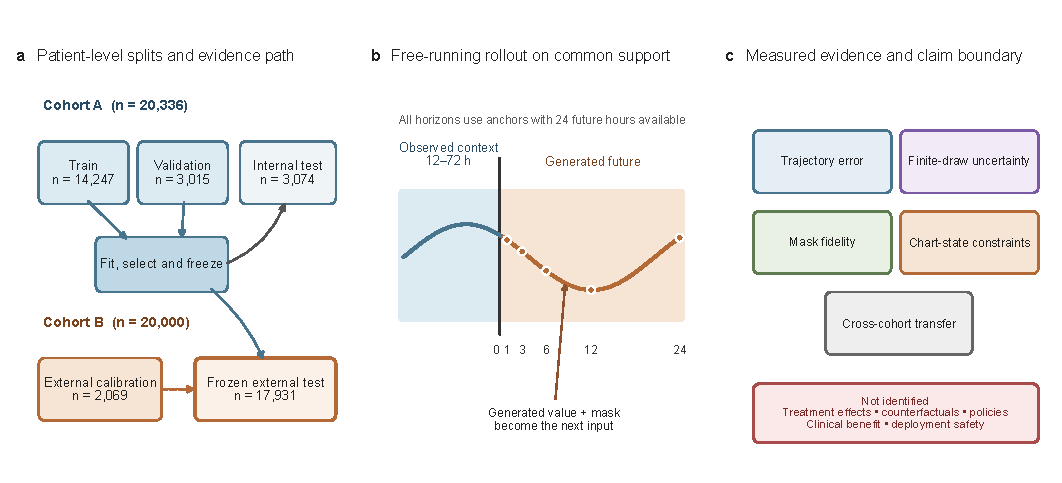
\includegraphics[width=0.98\textwidth]{figures/figure-1.pdf}
\caption{Evaluation design, free-running rollout, and claim boundary. Panel (a) shows the patient-disjoint development, internal-test, external-calibration, and frozen external-test partitions. The external-calibration partition can adjust predictive spread but cannot alter model parameters or select a model. Panel (b) shows the common-support free-running task: every reported horizon uses anchors with all 24 future hours available, and generated values and measurement masks become later inputs. Panel (c) distinguishes the evidence measured from claims that the observational passive-forecasting design does not identify.}
\label{fig:result-1}
\end{figure*}

\subsection{Variables and preprocessing}\label{variables-and-preprocessing}

The candidate feature set comprised 34 hourly physiological variables. A
variable was retained when its observation frequency was at least 5\% in the
cohort-A training partition. This yielded 24 variables: heart rate, oxygen
saturation, temperature, systolic, mean, and diastolic blood pressure,
respiratory rate, base excess, bicarbonate, inspired oxygen fraction, pH,
arterial carbon dioxide, arterial oxygen saturation, blood urea nitrogen,
chloride, creatinine, glucose, magnesium, phosphate, potassium, hematocrit,
hemoglobin, white blood-cell count, and platelets.

All medians, interquartile ranges, coverage decisions, and clipping statistics
were estimated from cohort-A training patients. Observed values were robustly
scaled. Missing values in model inputs were carried forward after a
training-median initialization and were accompanied by an observation mask and
hours since last measurement. Elapsed time since measurement was clipped at 24
hours and scaled to {[}0,1{]}. The ICU-time feature, rather than the patient
record, was capped at 72 hours and scaled to {[}0,1{]}. Imputed values were never
scored as observed targets.

\subsection{Forecasting task and common support}\label{forecasting-task-and-common-support}

For each eligible anchor, a model received up to 72 hours of history, with a
minimum context of 12 hours, and generated future values and measurement masks
at 1, 3, 6, 12, and 24 hours. The primary evaluation used free-running rollout:
sampled values and masks were recursively returned to the model rather than
replaced by future observations. The one-hour endpoint is a single generated
step from the real history. The protocol's proposed teacher-forced comparison
at longer horizons was deferred and is not represented as completed.

Every reported horizon used the same anchors. An anchor was eligible only when
all 24 future hours were available, and anchors were sampled every six hours.
Because value metrics exclude missing targets, the number of scored targets
and patients with at least one scored target still varies by horizon. Common
support therefore denotes identical anchor eligibility, not identical
horizon-specific observed-target support.

\subsection{Models}\label{models}

We evaluated three deterministic sanity baselines:

\begin{itemize}
\tightlist
\item
  last observation carried forward;
\item
  a training-cohort global median; and
\item
  a training-cohort median conditional on ICU hour.
\end{itemize}

A ridge vector autoregression used three lagged robust-scaled states and an
intercept. Its regularization coefficient was selected by validation-set
12-hour patient-macro normalized mean absolute error and was then frozen.

The probabilistic neural comparison comprised:

\begin{itemize}
\tightlist
\item
  a probabilistic GRU-D-style recurrent forecaster using values, masks, and
  time since measurement \cite{b3};
\item
  a causally masked Transformer forecaster with cached autoregressive inference
  \cite{b4}; and
\item
  a recurrent stochastic state-space model with a 32-dimensional latent state,
  adapted from latent-dynamics modeling principles \cite{b5}.
\end{itemize}

All neural models used a hidden size of 96, a Gaussian value head, and a
Bernoulli measurement-mask head. The Transformer used three layers, four
attention heads, and dropout 0.1; the recurrent models did not use an explicit
dropout layer. The resulting parameter counts differed by architecture and are
reported with the results. Models were optimized with AdamW at learning rate
0.0003, weight decay 0.00001, gradient clipping at 1.0, and batch size 64.
Training was limited to 20 epochs with validation early stopping. The objective
combined observed-value Gaussian negative log likelihood with mask
cross-entropy; the state-space model additionally used a weighted latent
Kullback-Leibler term. Training and validation objectives were averaged over
minibatches; publication outcomes use the separate patient-macro aggregation
defined below. Complete window sampling, loss weights, scale bounds,
checkpoint selection, and parameter counts are reported in Supplementary
Table S4.

Evaluation used batches of 128 patient-time anchors to reduce accelerator
kernel overhead; this setting did not change model parameters, support, or
metric definitions.

Each neural family was trained with seeds 20260912 through 20260916 under the
same data, maximum epoch count, stopping rule, optimizer settings, and
evaluation code. Architecture-specific parameter counts were not matched, so
comparisons are fixed-budget benchmarks of these implementations rather than
controlled mechanistic ablations or population-level model-family rankings.
All GRU-D and Transformer runs selected the maximum epoch 20, so longer
training could change their results. Ridge and neural models also used
different validation-selection objectives. Accelerator kernels may remain
nondeterministic, and seed-level results are retained rather than represented
as exact computational replicates.

\subsection{Probabilistic rollout and post-hoc spread adaptation}\label{probabilistic-rollout-and-post-hoc-spread-adaptation}

Twenty stochastic trajectories were generated for each patient-time anchor.
Point forecasts were the trajectory mean. Distributional performance was
evaluated from the 20-draw empirical trajectory distribution. The reported
90\% interval used linearly interpolated empirical 5th and 95th percentiles.
With 20 draws, those quantiles, the sample mean, CRPS, and the
sample-standard-deviation score include non-negligible Monte Carlo error and
do not directly characterize the infinite-draw model distribution. Under
exchangeable draws from a calibrated continuous distribution, the implemented
linearly interpolated interval has expected finite-sample coverage of
approximately 0.814 at 20 draws, 0.865 at 50 draws, and 0.882 at 100 draws,
rather than exactly 0.90.

The initial protocol anticipated a separate external-calibration analysis. The
exact horizon-wise scalar procedure was fixed after the implementation seed
and before the remaining seed matrix, so it is treated as a post-pilot
adaptation analysis. One nonnegative spread multiplier was fitted per horizon
on the external-calibration partition. For raw predictive samples
with mean \(\mu\), standard deviation \(\sigma\), and observed target \(y\), the
multiplier was

\[
s_h = \sqrt{\operatorname{mean}\left[\left((y-\mu)/\sigma\right)^2\right]}
\]

over observed targets at horizon \(h\). Spread-adapted samples were
\(\mu+s_h(x-\mu)\). This operation changed marginal spread only. It did not
change the point forecast, generated rollout states, predicted measurement
masks, or raw trajectory constraint counts.

The multiplier was fitted from the same 20-draw procedure by pooling observed
targets, whereas test outcomes were aggregated patient first. It therefore
targets pooled marginal spread, not variable-specific, patient-conditional,
joint, or measurement-mask calibration. It can compensate for both model
dispersion and finite-draw estimation and is not interpreted as a pure
correction of the underlying model distribution.

\subsection{Outcomes}\label{outcomes}

The primary descriptive outcomes were:

\begin{enumerate}
\def\labelenumi{\arabic{enumi}.}
\tightlist
\item
  patient-macro normalized mean absolute error at 12 hours;
\item
  patient-macro continuous ranked probability score at 12 hours;
\item
  area under the 1- to 24-hour rollout-degradation curve;
\item
  coverage of the empirical 5th- to 95th-percentile interval, with 0.90
  retained only as an infinite-draw reference;
\item
  prespecified constraint violations per 1,000 sampled rollout states;
\item
  relative degradation from internal to external testing; and
\item
  patient-macro measurement-mask Brier score.
\end{enumerate}

NMAE was absolute error after scaling each variable by the cohort-A training
interquartile range, averaged across scored variable-anchor targets within a
patient and then equally across patients. Secondary outcomes included
one-hour error, a moment-matched Gaussian negative log score, interval width,
and variable-specific metrics. The negative log
score used the empirical trajectory mean and standard deviation and is not the
exact likelihood of a generally non-Gaussian rollout distribution. CRPS was
used as a proper scoring rule for the empirical predictive distribution \cite{b6};
interval coverage and spread adaptation were interpreted as finite-draw
uncertainty diagnostics rather than substitutes for accuracy \cite{b7,b8}.

Prespecified chart-state checks included systolic pressure greater than or
equal to mean
pressure greater than or equal to diastolic pressure, oxygen saturation in
{[}0,100{]}, arterial oxygen saturation in {[}0,100{]}, and inspired oxygen fraction
in {[}0,1{]}. The primary constraint metric used the actual rollout state after
applying the sampled measurement mask and carrying unmeasured values forward.
Violations in every decoder emission were retained as a separate diagnostic.
Because masks can update pressure components at different simulated times, a
rollout-state ordering violation may reflect asynchronous carry-forward
inconsistency rather than an impossible simultaneous measurement. No matched
observed-data reference rate was estimated. Both diagnostics were calculated
from the raw trajectory so that spread scaling could not alter them.

\subsection{Statistical analysis}\label{statistical-analysis}

All comparisons use identical patient-time anchors within a split. Metrics are
aggregated across anchors and observed variables within each patient and then
equally across patients. Neural patient metrics are averaged over the five
fixed trained instances; across-seed standard deviation and range are reported
separately. The primary estimand therefore concerns these five instances, not
the full distribution of possible training runs.

Patient-bootstrap intervals resample patients after fixed-seed averaging.
Paired bootstrap contrasts are restricted to the frozen 12-hour NMAE
comparisons on the same patients. Internal and external cohorts contain
different patients, so cross-cohort intervals resample each cohort
independently. Rank stability is described by Spearman correlation and the
fraction of model pairs whose order reverses across horizons or cohorts.
Patient-bootstrap intervals quantify patient sampling conditional on the five
fitted neural instances; they do not include training-run uncertainty.
Across-seed standard deviations describe those instances separately.

For horizon-level metric \(M_h\), the normalized rollout area is the
trapezoidal area across 1, 3, 6, 12, and 24 hours divided by 23 hours. External
degradation is reported as \(M_B-M_A\) and
\(100(M_B-M_A)/M_A\), where \(A\) is internal and \(B\) is zero-shot external.

The initial protocol proposed multiplicity control but did not define exact
null contrasts. We therefore emphasize effect sizes and 95\% bootstrap
intervals and do not present retrospectively specified \(p\)-values as
confirmatory tests. Analyses formalized after the implementation seed are
labeled exploratory or post-pilot. A sensitivity analysis excludes the
inspected implementation seed.

Because empirical quantiles and sample-based proper scores can depend on Monte
Carlo count, a post-analysis numerical sensitivity reran the implementation
seed with 20, 50, and 100 trajectories on the same hashed subset of 1,000
external-test patients. This analysis assessed estimator stability rather than
training-seed uncertainty and did not replace the prespecified five-seed,
20-trajectory primary analysis. The three counts used separate fixed random
streams rather than a repeated-stream convergence design.

Missing targets do not enter value metrics. Mask metrics use all target
variables. No test-set result is used to select a model or adjust a
hyperparameter.

\subsection{Reproducibility}\label{reproducibility}

The local reproducibility package records the dataset fingerprint, deterministic patient
split, selected variables, training configuration, model checkpoints,
seed-level training histories, raw patient-level metrics, spread-adaptation
artifacts, and scripts used to generate summary tables. Source patient files
are not redistributed. An immutable reviewer-accessible release remains a
submission gate.

\section{Results}\label{results}

\subsection{Cohort and evaluation support}\label{cohort-and-evaluation-support}

After applying the 12-hour minimum context and 24-hour common-support rule,
1,841 internal-test and 10,622 external-test patients contributed at least one
eligible anchor, yielding 5,143 and 30,450 common anchors, respectively. Across
the 24 retained variables, the observed-value fraction was 28.36\% in the full
internal-test records and 26.04\% in the full external-test records. Effective
value-metric support varied with observed targets: internal support ranged
from 1,810 patients and 36,216 targets at one hour to 1,773 and 32,924 at 24
hours; external support ranged from 10,245 patients and 198,911 targets to
10,162 and 192,680. The 12-hour paired comparisons used 1,806 internal and
10,178 external patients.

\subsection{One-step and free-running accuracy}\label{one-step-and-free-running-accuracy}

The one-hour and long-horizon comparisons did not select the same model
(Figure 2). Externally, ridge had the lowest one-hour NMAE (0.3610), followed
by the Transformer (0.3768), GRU-D (0.3770), and persistence (0.3853). At 12
hours, the Transformer (0.5207) and GRU-D (0.5216) were better than ridge
(0.5301); the same ordering remained at 24 hours (0.5591, 0.5607, and 0.5862).
The state-space model reached NMAE 0.6220 at 12 hours.

At 12 hours, the external paired contrast was -0.0093 (95\% patient-bootstrap
interval conditional on the five fitted instances,
-0.0114 to -0.0074) for Transformer versus ridge and -0.0085 (-0.0102 to
-0.0068) for GRU-D versus ridge. GRU-D minus Transformer was 0.0008 (-0.0000
to 0.0017), compatible with essentially tied performance. Ridge was better
than persistence by -0.0452 (-0.0488 to -0.0414), while the state-space model
was worse than ridge by 0.0919 (0.0896 to 0.0942).

The prespecified external NMAE rollout-area summary was 0.5083 (across-seed
SD 0.0038) for the Transformer, 0.5087 (0.0016) for GRU-D, 0.5158 for ridge,
0.5516 for persistence, 0.6105 (0.0054) for the state-space model, 0.6652 for
the hourly median, and 0.6656 for the global median. Excluding the inspected
implementation seed did not change the main pattern: 12-hour NMAE was 0.5213
for the Transformer, 0.5216 for GRU-D, and 0.6234 for the state-space model.

Original-unit 12-hour errors were heterogeneous across variables
(Supplementary Table S1). The Transformer versus ridge MAE was 9.65 versus
9.84 for heart rate, 1.96 versus 2.03 for oxygen saturation, 15.28 versus
16.74 for systolic pressure, and 10.33 versus 11.38 for mean pressure. Ridge
was better for temperature (0.502 versus 0.511), creatinine (0.403 versus
0.442), glucose (29.55 versus 30.87), and white-cell count (2.58 versus
2.88). The aggregate NMAE advantage was therefore not uniform across clinical
variables, and no minimum clinically important difference was defined.

\begin{figure*}[!t]
\centering
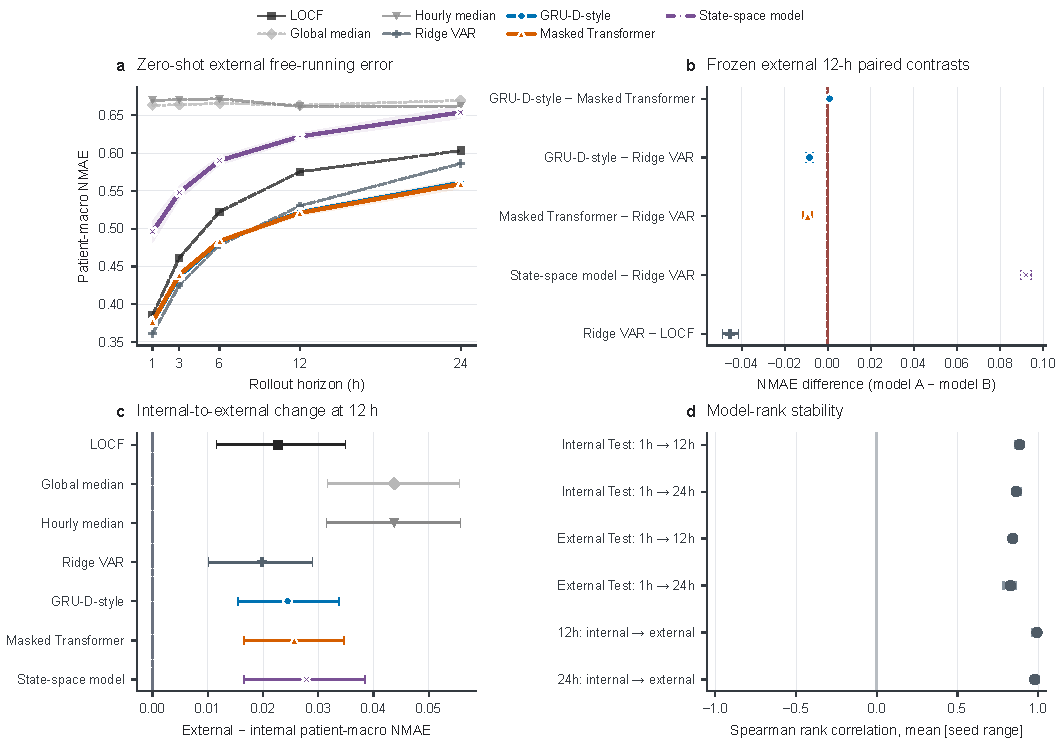
\includegraphics[width=0.98\textwidth]{figures/figure-2.pdf}
\caption{Free-running accuracy and transfer. (a) Zero-shot external NMAE by horizon; ribbons show one across-seed SD for neural models. (b) Frozen external 12-hour patient-bootstrap contrasts conditional on five fitted instances; negative values favor model A. (c) Internal-to-external 12-hour change with independently resampled patient-bootstrap intervals. (d) Model-rank correlations among seven models; bars show seed ranges.}
\label{fig:result-2}
\end{figure*}

\subsection{Finite-draw uncertainty and spread adaptation}\label{finite-draw-uncertainty-and-spread-adaptation}

Under the 20-draw primary procedure, 12-hour external 90\% coverage was 0.8422
for GRU-D, 0.8673 for the Transformer, and 0.4981 for the state-space model
(Figure 3). Spread adaptation increased coverage to 0.8841, 0.8866, and
0.8784, respectively. These changes describe the implemented empirical
interval and are not interpreted as reductions in intrinsic model-calibration
error.

Mean interval width increased from 1.9116 to 2.1839 scaled units for GRU-D,
2.1120 to 2.2555 for the Transformer, and 1.0269 to 2.6629 for the state-space
model. Gaussian negative log score improved from 1.1100 to 1.0874, 1.0927 to
1.0886, and 3.2856 to 1.2795. CRPS became slightly worse for GRU-D (0.3850 to
0.3885) and the Transformer (0.3851 to 0.3874) but improved for the
state-space model (0.4957 to 0.4706). Spread adaptation therefore altered the
20-draw empirical distribution without making the state-space model
competitive on accuracy. The maximum
patient-level raw-versus-adapted NMAE difference was
\(4.768\times10^{-7}\), and mask-Brier difference was zero.

\begin{figure*}[!t]
\centering
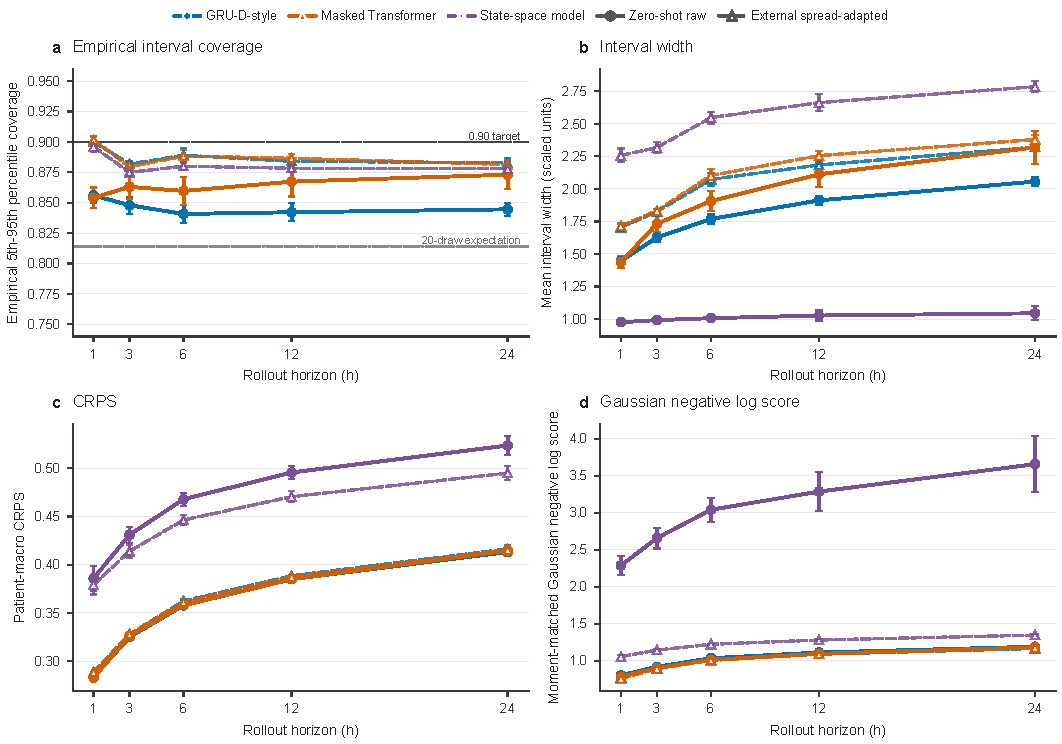
\includegraphics[width=0.98\textwidth]{figures/figure-3.pdf}
\caption{External 20-draw uncertainty before and after spread adaptation. Panels show (a) empirical 5th- to 95th-percentile coverage, (b) interval width, (c) CRPS, and (d) moment-matched Gaussian negative log score. Circles are zero-shot results and triangles are horizon-specific spread scaling fitted on external-calibration data with the same 20-draw procedure. Error bars show across-seed SDs, not patient-bootstrap intervals. The dotted line is the infinite-draw 0.90 target; the dash-dotted line is the approximately 0.814 expectation for the implemented 20-draw quantile rule under exchangeability. These panels characterize the finite-draw procedure rather than the infinite-draw model distribution.}
\label{fig:result-3}
\end{figure*}

\subsection{Observation-process fidelity}\label{observation-process-fidelity}

At 12 hours, external mask Brier scores were 0.0617 for GRU-D, 0.0628 for the
Transformer, and 0.0645 for the state-space model; internal values were
0.0730, 0.0725, and 0.0797. The lower external scores occurred with lower
measurement prevalence and should not be read as improved patient-state
transport. At 12 hours within each cohort, the state-space model had both the
weakest value forecast and the weakest observation-process forecast.

\subsection{Prespecified chart-state constraint diagnostics}\label{prespecified-chart-state-constraint-diagnostics}

Accuracy and narrow constraint consistency gave different rankings (Figure 4).
At 12
hours, GRU-D and the Transformer produced 161.1 and 204.9 pressure-order
violations per 1,000 rollout states, compared with 2.50 for the state-space
model, 0.624 for ridge, 5.32 for persistence, and zero for median baselines.
For GRU-D, Transformer, and the state-space model, respectively, rates were
123.0, 158.8, and 11.2 for oxygen-saturation bounds; 50.8, 49.4, and 70.3 for
arterial-oxygen-saturation bounds; and 5.7, 8.3, and 0.2 for inspired-oxygen
fraction.

Low violation counts did not imply useful dynamics: the state-space model had
worse NMAE and uncertainty, and median forecasts satisfied pressure ordering
by construction. Conversely, the two most accurate long-horizon models often
violated the pressure-order rule. Because mask-gated values can have different
carry-forward ages and no matched observed-chart reference was computed, these
rates are descriptive consistency diagnostics, not estimates of impossible
simultaneous physiology or clinical safety.

\begin{figure*}[!t]
\centering
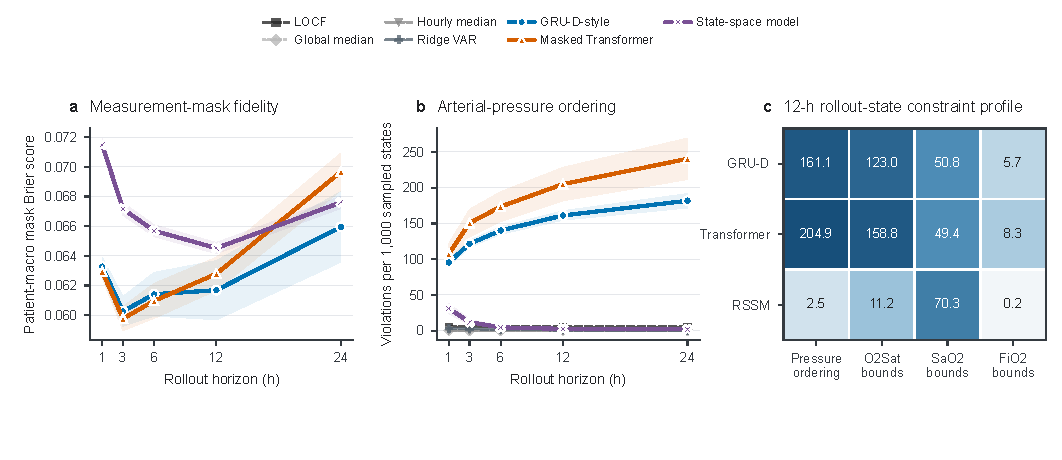
\includegraphics[width=0.98\textwidth]{figures/figure-4.pdf}
\caption{Observation-process and chart-state constraint diagnostics. (a) External mask Brier score. (b) Arterial-pressure ordering violations in actual rollout states. (c) Four prespecified 12-hour constraints for neural models. Rates are per 1,000 sampled states; heat-map color encodes frequency, not clinical severity. Ribbons in panels (a) and (b) show one across-seed SD.}
\label{fig:result-4}
\end{figure*}

\subsection{Cross-cohort degradation and ranking stability}\label{cross-cohort-degradation-and-ranking-stability}

Every model had higher 12-hour NMAE externally. Relative degradation was 3.9\%
(95\% interval, 2.0\% to 5.7\%) for ridge, 4.9\% (3.1\% to 6.9\%) for GRU-D, 5.2\%
(3.3\% to 7.1\%) for the Transformer, 4.7\% (2.7\% to 6.6\%) for the state-space
model, and 4.1\% (2.1\% to 6.4\%) for persistence.

Cross-cohort rank order among seven models remained stable: mean Spearman
correlation was 0.993 at
12 hours and 0.979 at 24 hours. Horizon transfer was less complete. External
one-to-12-hour correlation was 0.843, with 16.2\% of model pairs reversing;
one-to-24-hour values were 0.829 and 17.1\%.

Trajectory-count sensitivity qualified raw uncertainty estimates. On the same
1,000 external patients and implementation seed, 12-hour coverage increased
from 0.8401 with 20 trajectories to 0.8945 with 100 for GRU-D and from 0.8632
to 0.9195 for the Transformer. Their CRPS and sample-mean NMAE also decreased.
The state-space model increased only from 0.4978 to 0.5491 and remained
underdispersed. Pressure-order rates were comparatively stable.

\begin{figure*}[!t]
\centering
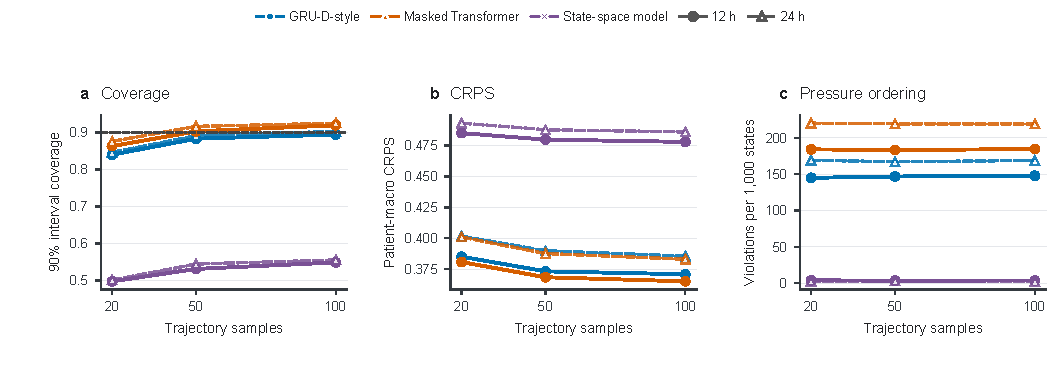
\includegraphics[width=0.98\textwidth]{figures/figure-5.pdf}
\caption{Limited Monte Carlo-count sensitivity. Coverage, CRPS, and pressure-order violations for 20, 50, and 100 trajectories on the same hashed subset of 1,000 external patients. This analysis uses one trained implementation seed, separate fixed streams, and no repeated-stream Monte Carlo intervals. Circles and triangles denote 12- and 24-hour horizons.}
\label{fig:result-5}
\end{figure*}

\subsection{Descriptive zero-shot external-test result table}\label{descriptive-zero-shot-external-test-result-table}

\begin{table*}[!t]
\centering
\caption{Descriptive zero-shot external-test results. Neural values are mean (across-seed standard deviation).}
\label{tab:external-results}
\resizebox{\textwidth}{!}{%
\begin{tabular}{lrrrrrrr}
\toprule
Model & 1 h NMAE & 12 h NMAE & 24 h NMAE & 12 h CRPS & Empirical coverage & Mask Brier & Pressure violations/1,000 \\
\midrule
Last observation carried forward & 0.3853 & 0.5753 & 0.6033 & NA & NA & NA & 5.320 \\
Global median & 0.6634 & 0.6634 & 0.6698 & NA & NA & NA & 0.000 \\
Hourly median & 0.6699 & 0.6617 & 0.6624 & NA & NA & NA & 0.000 \\
Ridge vector autoregression & 0.3610 & 0.5301 & 0.5862 & NA & NA & NA & 0.624 \\
Probabilistic GRU-D-style model & 0.3770 (0.0010) & 0.5216 (0.0013) & 0.5607 (0.0030) & 0.3850 (0.0008) & 0.8422 (0.0073) & 0.0617 (0.0020) & 161.067 (6.562) \\
Causally masked Transformer & 0.3768 (0.0016) & 0.5207 (0.0038) & 0.5591 (0.0062) & 0.3851 (0.0031) & 0.8673 (0.0123) & 0.0628 (0.0011) & 204.920 (23.372) \\
Recurrent state-space model & 0.4958 (0.0142) & 0.6220 (0.0047) & 0.6539 (0.0081) & 0.4957 (0.0065) & 0.4981 (0.0149) & 0.0645 (0.0004) & 2.496 (1.254) \\
\bottomrule
\end{tabular}%
}
\end{table*}

Baseline values use external-test patient-macro means on the common anchor set.
Neural entries are mean (across-seed standard deviation). The displayed
constraint rate is the 12-hour arterial-pressure ordering rate.

\section{Discussion}\label{discussion}

This study yields four main findings. First, one-step accuracy did not fully
determine free-running performance. Ridge was best at one hour, but GRU-D and
the Transformer were better at 12 and 24 hours and essentially tied
externally. Long-horizon rollout changed the conclusion without establishing
an architectural winner.

Second, stochastic architecture did not guarantee useful uncertainty. The
state-space model contained latent randomness yet produced narrow intervals,
approximately 50\% 12-hour coverage, and the worst CRPS and NMAE. Spread
scaling changed finite-draw coverage and negative log score but not the learned
mean trajectory. For all models, the 20-draw multiplier combines model spread
with Monte Carlo estimation and cannot be interpreted as a pure calibration
correction.

Third, the most accurate neural models had the highest pressure-order
violation rates in mask-gated chart states. Favorable average error can
therefore coexist with failure of a narrow prespecified consistency rule. The
converse also failed: state-space and median models had fewer violations
without useful overall accuracy. These checks must be reported beside error,
not used as a validity or safety certificate. Constrained decoding is a
plausible next intervention, but its effects require direct testing.

Fourth, cohort shift increased error but barely changed rankings. This negative
finding narrows the original hypothesis: here, horizon shift mattered more
than cohort shift for comparative order. Stable ranking does not make external
error acceptable, so frozen external testing remains necessary.

The trajectory-count sensitivity changes the interpretation of raw coverage.
With 20 samples, empirical 5th and 95th percentiles are not a finite-sample
90\% prediction interval, and sample means, CRPS, and Gaussian scores retain
simulation error. At 100 samples, GRU-D approached nominal coverage and the
Transformer moved slightly above it on the tested subset. The state-space
model remained far below nominal. Because the sensitivity used one trained
seed and separate single streams, it demonstrates dependence rather than
convergence. Future evaluations should use finite-sample-valid intervals,
repeated nested streams, or analytic summaries where available.

Together, the results support an evaluation bundle rather than a new
architecture claim: common-eligibility free-running curves, proper scores,
finite-draw uncertainty with Monte Carlo sensitivity, observation-process
fidelity, prespecified chart-state constraints, and frozen external testing.
This bundle assesses a simulator of the recorded passive chart process; it
does not establish latent physiological, causal, or clinical validity.

\subsection{Limitations}\label{limitations}

The study uses one challenge dataset with two source cohorts rather than
prospective deployment data. Cohort B shares the challenge schema, so it tests
transfer but not general deployment validity. Sparse observation limits
variable-specific precision. The 20-trajectory primary analysis mixes model
behavior with Monte Carlo error, as the sensitivity analysis demonstrates.
Spread adaptation is pooled and scalar by horizon, not conditional or joint.
Constraint rates lack a matched observed-chart reference, patient-clustered
intervals, and clinician validation; pressure components may have different
carry-forward ages. Variable-level original-unit errors were descriptive and
lacked clinician-validated importance thresholds, so small aggregate NMAE
differences have no defined minimum clinically important interpretation.
Models omit static variables, treatment actions,
discharge, and death. Parameter counts differ, hyperparameter exploration was
limited, GRU-D and Transformer training ended at the epoch cap, and
architecture differences cannot be attributed to one mechanism.

\section{Conclusion}\label{conclusion}

One-step error, long-horizon accuracy, finite-draw uncertainty, and narrow
chart-state constraints did not identify the same implementation. Ridge was
strongest at one hour; GRU-D and the Transformer were strongest at 12 and 24
hours but had high pressure-order violation rates; and the stochastic
state-space model was inaccurate and robustly underdispersed. Spread scaling
changed the 20-draw empirical distribution without repairing dynamics, while
cohort shift raised errors but left rankings mostly stable. Medical
world-model claims should therefore be matched to free-running, uncertainty,
constraint, and transfer evidence reported together. The present evidence is
limited to passive chart-process forecasting.

\section{Data and Code Availability}\label{data-and-code-availability}

The source dataset is publicly available from PhysioNet under its published
terms. The local reproducibility package contains code, split hashes,
aggregate data fingerprints, trained checkpoints, spread-adaptation artifacts,
patient-level derived metrics, source data for figures, and result tables; it
does not redistribute source patient files. A stable immutable release is
required before submission.

\section{Ethics}\label{ethics}

This study uses deidentified public data and performs retrospective model
evaluation only. The research team must confirm the applicable institutional
determination before submission.

\section{Funding}\label{funding}

Funding information is withheld for anonymous review.

\section{Declaration of Competing Interest}\label{declaration-of-competing-interest}

Competing-interest information is withheld for anonymous review.

\section{Declaration of Generative AI and AI-Assisted Technologies}\label{declaration-of-generative-ai-and-ai-assisted-technologies}

OpenAI Codex was used for code assistance, evidence organization, drafting, and
language revision under author supervision. The authors will verify all
methods, results, citations, and interpretations and take full responsibility
for the final manuscript.

\balance
\begin{thebibliography}{00}
\bibitem{b1} Reyna MA, Josef CS, Jeter R, et al. Early Prediction of Sepsis From Clinical Data: The PhysioNet/Computing in Cardiology Challenge 2019. Critical Care Medicine. 2020;48(2):210-217. doi:10.1097/CCM.0000000000004145.
\bibitem{b2} Reyna MA, Josef CS, Jeter R, et al. Early Prediction of Sepsis from Clinical Data: The PhysioNet/Computing in Cardiology Challenge 2019. PhysioNet. 2019. Version 1.0.0. doi:10.13026/v64v-d857.
\bibitem{b3} Che Z, Purushotham S, Cho K, Sontag D, Liu Y. Recurrent Neural Networks for Multivariate Time Series with Missing Values. Scientific Reports. 2018;8:6085. doi:10.1038/s41598-018-24271-9.
\bibitem{b4} Vaswani A, Shazeer N, Parmar N, et al. Attention Is All You Need. Advances in Neural Information Processing Systems. 2017;30.
\bibitem{b5} Hafner D, Lillicrap T, Fischer I, et al. Learning Latent Dynamics for Planning from Pixels. In: Proceedings of the 36th International Conference on Machine Learning. PMLR; 2019:2555-2565.
\bibitem{b6} Gneiting T, Raftery AE. Strictly Proper Scoring Rules, Prediction, and Estimation. Journal of the American Statistical Association. 2007;102(477):359-378. doi:10.1198/016214506000001437.
\bibitem{b7} Kuleshov V, Fenner N, Ermon S. Accurate Uncertainties for Deep Learning Using Calibrated Regression. In: Proceedings of the 35th International Conference on Machine Learning. PMLR; 2018:2796-2804.
\bibitem{b8} Ovadia Y, Fertig E, Ren J, et al. Can You Trust Your Model's Uncertainty? Evaluating Predictive Uncertainty Under Dataset Shift. Advances in Neural Information Processing Systems. 2019;32.
\bibitem{b9} Rubanova Y, Chen RTQ, Duvenaud D. Latent Ordinary Differential Equations for Irregularly-Sampled Time Series. Advances in Neural Information Processing Systems. 2019;32.
\bibitem{b10} Arık SÖ, et al. EHR-Safe: Generating High-Fidelity and Privacy-Preserving Synthetic Electronic Health Records. npj Digital Medicine. 2023;6:141. doi:10.1038/s41746-023-00888-7.
\bibitem{b11} Theodorou B, Xiao C, Sun J. Synthesize High-Dimensional Longitudinal Electronic Health Records via Hierarchical Autoregressive Language Model. Nature Communications. 2023;14:5305. doi:10.1038/s41467-023-41093-0.
\bibitem{b12} Li J, et al. External Validation and Evaluation of Algorithms for Patient Deterioration Prediction Using a National Dataset. Scientific Reports. 2023;13:9240. doi:10.1038/s41598-023-36318-1.
\end{thebibliography}

\end{document}
